% Options for packages loaded elsewhere
% Options for packages loaded elsewhere
\PassOptionsToPackage{unicode}{hyperref}
\PassOptionsToPackage{hyphens}{url}
\PassOptionsToPackage{dvipsnames,svgnames,x11names}{xcolor}
%
\documentclass[
  letterpaper,
  DIV=11,
  numbers=noendperiod]{scrartcl}
\usepackage{xcolor}
\usepackage{amsmath,amssymb}
\setcounter{secnumdepth}{5}
\usepackage{iftex}
\ifPDFTeX
  \usepackage[T1]{fontenc}
  \usepackage[utf8]{inputenc}
  \usepackage{textcomp} % provide euro and other symbols
\else % if luatex or xetex
  \usepackage{unicode-math} % this also loads fontspec
  \defaultfontfeatures{Scale=MatchLowercase}
  \defaultfontfeatures[\rmfamily]{Ligatures=TeX,Scale=1}
\fi
\usepackage{lmodern}
\ifPDFTeX\else
  % xetex/luatex font selection
\fi
% Use upquote if available, for straight quotes in verbatim environments
\IfFileExists{upquote.sty}{\usepackage{upquote}}{}
\IfFileExists{microtype.sty}{% use microtype if available
  \usepackage[]{microtype}
  \UseMicrotypeSet[protrusion]{basicmath} % disable protrusion for tt fonts
}{}
\makeatletter
\@ifundefined{KOMAClassName}{% if non-KOMA class
  \IfFileExists{parskip.sty}{%
    \usepackage{parskip}
  }{% else
    \setlength{\parindent}{0pt}
    \setlength{\parskip}{6pt plus 2pt minus 1pt}}
}{% if KOMA class
  \KOMAoptions{parskip=half}}
\makeatother
% Make \paragraph and \subparagraph free-standing
\makeatletter
\ifx\paragraph\undefined\else
  \let\oldparagraph\paragraph
  \renewcommand{\paragraph}{
    \@ifstar
      \xxxParagraphStar
      \xxxParagraphNoStar
  }
  \newcommand{\xxxParagraphStar}[1]{\oldparagraph*{#1}\mbox{}}
  \newcommand{\xxxParagraphNoStar}[1]{\oldparagraph{#1}\mbox{}}
\fi
\ifx\subparagraph\undefined\else
  \let\oldsubparagraph\subparagraph
  \renewcommand{\subparagraph}{
    \@ifstar
      \xxxSubParagraphStar
      \xxxSubParagraphNoStar
  }
  \newcommand{\xxxSubParagraphStar}[1]{\oldsubparagraph*{#1}\mbox{}}
  \newcommand{\xxxSubParagraphNoStar}[1]{\oldsubparagraph{#1}\mbox{}}
\fi
\makeatother


\usepackage{longtable,booktabs,array}
\usepackage{calc} % for calculating minipage widths
% Correct order of tables after \paragraph or \subparagraph
\usepackage{etoolbox}
\makeatletter
\patchcmd\longtable{\par}{\if@noskipsec\mbox{}\fi\par}{}{}
\makeatother
% Allow footnotes in longtable head/foot
\IfFileExists{footnotehyper.sty}{\usepackage{footnotehyper}}{\usepackage{footnote}}
\makesavenoteenv{longtable}
\usepackage{graphicx}
\makeatletter
\newsavebox\pandoc@box
\newcommand*\pandocbounded[1]{% scales image to fit in text height/width
  \sbox\pandoc@box{#1}%
  \Gscale@div\@tempa{\textheight}{\dimexpr\ht\pandoc@box+\dp\pandoc@box\relax}%
  \Gscale@div\@tempb{\linewidth}{\wd\pandoc@box}%
  \ifdim\@tempb\p@<\@tempa\p@\let\@tempa\@tempb\fi% select the smaller of both
  \ifdim\@tempa\p@<\p@\scalebox{\@tempa}{\usebox\pandoc@box}%
  \else\usebox{\pandoc@box}%
  \fi%
}
% Set default figure placement to htbp
\def\fps@figure{htbp}
\makeatother





\setlength{\emergencystretch}{3em} % prevent overfull lines

\providecommand{\tightlist}{%
  \setlength{\itemsep}{0pt}\setlength{\parskip}{0pt}}



 


\KOMAoption{captions}{tableheading}
\makeatletter
\@ifpackageloaded{caption}{}{\usepackage{caption}}
\AtBeginDocument{%
\ifdefined\contentsname
  \renewcommand*\contentsname{Table of contents}
\else
  \newcommand\contentsname{Table of contents}
\fi
\ifdefined\listfigurename
  \renewcommand*\listfigurename{List of Figures}
\else
  \newcommand\listfigurename{List of Figures}
\fi
\ifdefined\listtablename
  \renewcommand*\listtablename{List of Tables}
\else
  \newcommand\listtablename{List of Tables}
\fi
\ifdefined\figurename
  \renewcommand*\figurename{Figure}
\else
  \newcommand\figurename{Figure}
\fi
\ifdefined\tablename
  \renewcommand*\tablename{Table}
\else
  \newcommand\tablename{Table}
\fi
}
\@ifpackageloaded{float}{}{\usepackage{float}}
\floatstyle{ruled}
\@ifundefined{c@chapter}{\newfloat{codelisting}{h}{lop}}{\newfloat{codelisting}{h}{lop}[chapter]}
\floatname{codelisting}{Listing}
\newcommand*\listoflistings{\listof{codelisting}{List of Listings}}
\makeatother
\makeatletter
\makeatother
\makeatletter
\@ifpackageloaded{caption}{}{\usepackage{caption}}
\@ifpackageloaded{subcaption}{}{\usepackage{subcaption}}
\makeatother
\usepackage{bookmark}
\IfFileExists{xurl.sty}{\usepackage{xurl}}{} % add URL line breaks if available
\urlstyle{same}
\hypersetup{
  pdftitle={Computational Notebooks in Python, R, and Stata},
  pdfauthor={Carlos Mendez},
  pdfkeywords={computational notebooks, reproducible
research, Python, R, Stata, data science},
  colorlinks=true,
  linkcolor={blue},
  filecolor={Maroon},
  citecolor={Blue},
  urlcolor={Blue},
  pdfcreator={LaTeX via pandoc}}


\title{Computational Notebooks in Python, R, and Stata}
\usepackage{etoolbox}
\makeatletter
\providecommand{\subtitle}[1]{% add subtitle to \maketitle
  \apptocmd{\@title}{\par {\large #1 \par}}{}{}
}
\makeatother
\subtitle{A Multi-Language Guide to Data Science Workflows}
\author{Carlos Mendez}
\date{2026-03-09}
\begin{document}
\maketitle
\begin{abstract}
This document introduces computational notebooks as a practical tool for
data science across three programming languages: Python, R, and Stata.
Through five companion notebooks, we demonstrate how Jupyter-based
environments support reproducible workflows ranging from exploratory
data analysis to machine learning and causal inference. The first three
notebooks present a common data exploration task implemented
independently in Python, R, and Stata, illustrating how each language
handles data generation, visualization, and summary statistics within
the same notebook platform. The fourth notebook introduces Random Forest
regression for predicting Bolivia's Municipal Sustainable Development
Index from satellite image embeddings. The fifth notebook demonstrates
Double Machine Learning for causal inference using the Pennsylvania
Reemployment Bonus experiment. Together, these notebooks provide a
hands-on reference for researchers and students working across multiple
computational environments.
\end{abstract}


\section{Introduction}\label{sec-introduction}

Computational notebooks have become a standard tool for reproducible
data science, combining code, output, and narrative in a single
document. While Python dominates the Jupyter ecosystem, researchers in
the social sciences and economics often work in R or Stata. This
document demonstrates that all three languages can be used effectively
within Jupyter notebooks, and that the same analytical tasks can be
accomplished across environments.

The companion notebooks use data from the
\href{https://github.com/quarcs-lab/ds4bolivia}{DS4Bolivia} project as a
running example. The dataset covers 339 Bolivian municipalities and
includes the Municipal Sustainable Development Index (IMDS),
64-dimensional satellite image embeddings, and regional identifiers.

The five notebooks are organized as follows:

\begin{itemize}
\tightlist
\item
  \href{notebooks/notebook-01.ipynb}{N1: Sample Data Exploration} ---
  Exploratory data analysis in Python
\item
  \href{notebooks/notebook-02.ipynb}{N2: Sample R Analysis} --- The same
  exploration in R
\item
  \href{notebooks/notebook-03.ipynb}{N3: Sample Stata Analysis} --- The
  same exploration in Stata
\item
  \href{notebooks/notebook-04.ipynb}{N4: Introduction to Machine
  Learning --- Random Forest Regression} --- Predicting sustainable
  development from satellite embeddings
\item
  \href{notebooks/notebook-05.ipynb}{N5: Introduction to Causal
  Inference --- Double Machine Learning} --- Estimating causal effects
  with debiased ML methods
\end{itemize}

Each section below introduces one notebook, summarizes its content, and
embeds selected figures and tables. Readers are encouraged to open the
full notebooks for complete code and discussion.

\section{Data Exploration in Python}\label{sec-python}

The first notebook (\href{notebooks/notebook-01.ipynb}{N1: Sample Data
Exploration}) demonstrates a standard exploratory data analysis workflow
in Python. It generates a synthetic dataset of 80 regions grouped into
four geographic clusters, each with simulated GDP per capita and life
expectancy values. The notebook illustrates how to set up a reproducible
environment using a shared configuration file (\texttt{config.py}),
create publication-quality visualizations with Matplotlib and Seaborn,
and compute summary statistics with Pandas.

The scatter plot below shows the relationship between GDP per capita and
life expectancy across the simulated regions, colored by geographic
cluster.

\begin{figure}[H]

\centering{

\pandocbounded{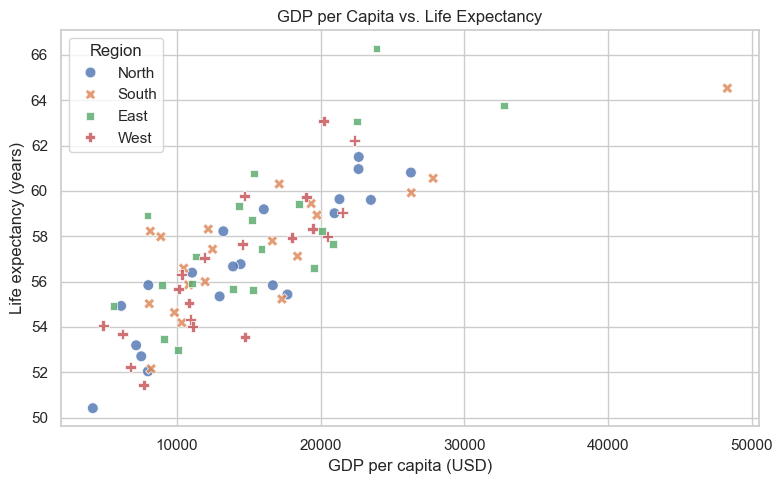
\includegraphics[keepaspectratio]{index_files/figure-latex/notebooks-notebook-01-fig-sample-output-1.png}}

}

\caption{\label{fig-sample}Synthetic regional indicators: GDP per capita
vs.~life expectancy across 80 simulated regions, colored by geographic
cluster.}

\end{figure}%

The following table reports summary statistics by region.

\begin{longtable}[]{@{}
  >{\raggedright\arraybackslash}p{(\linewidth - 12\tabcolsep) * \real{0.0488}}
  >{\raggedleft\arraybackslash}p{(\linewidth - 12\tabcolsep) * \real{0.1512}}
  >{\raggedleft\arraybackslash}p{(\linewidth - 12\tabcolsep) * \real{0.1463}}
  >{\raggedleft\arraybackslash}p{(\linewidth - 12\tabcolsep) * \real{0.1561}}
  >{\raggedleft\arraybackslash}p{(\linewidth - 12\tabcolsep) * \real{0.1659}}
  >{\raggedleft\arraybackslash}p{(\linewidth - 12\tabcolsep) * \real{0.1610}}
  >{\raggedleft\arraybackslash}p{(\linewidth - 12\tabcolsep) * \real{0.1707}}@{}}

\caption{\label{tbl-summary}Summary statistics by region.}

\tabularnewline

\toprule\noalign{}
\begin{minipage}[b]{\linewidth}\raggedright
Region
\end{minipage} & \begin{minipage}[b]{\linewidth}\raggedleft
GDP per capita (USD) (mean)
\end{minipage} & \begin{minipage}[b]{\linewidth}\raggedleft
GDP per capita (USD) (std)
\end{minipage} & \begin{minipage}[b]{\linewidth}\raggedleft
GDP per capita (USD) (count)
\end{minipage} & \begin{minipage}[b]{\linewidth}\raggedleft
Life expectancy (years) (mean)
\end{minipage} & \begin{minipage}[b]{\linewidth}\raggedleft
Life expectancy (years) (std)
\end{minipage} & \begin{minipage}[b]{\linewidth}\raggedleft
Life expectancy (years) (count)
\end{minipage} \\
\midrule\noalign{}
\endhead
\bottomrule\noalign{}
\endlastfoot
East & 15607.9 & 6499.5 & 20 & 58.1 & 3.4 & 20 \\
North & 14709 & 6638.8 & 20 & 56.7 & 3.1 & 20 \\
South & 16113.3 & 9541.1 & 20 & 57.5 & 2.8 & 20 \\
West & 13787 & 5498.2 & 20 & 56.7 & 3.2 & 20 \\

\end{longtable}

This notebook serves as a template that researchers can adapt to their
own datasets. The key takeaway is the basic workflow: load data,
visualize distributions and relationships, and summarize key variables
--- all within a single reproducible document.

\section{Data Exploration in R}\label{sec-r}

The second notebook (\href{notebooks/notebook-02.ipynb}{N2: Sample R
Analysis}) replicates the same exploratory analysis using R. It
demonstrates how to run R code inside a Jupyter notebook using the
IRkernel, generate equivalent visualizations with ggplot2, and produce
formatted tables with \texttt{knitr::kable()}.

The scatter plot below shows the same GDP-life expectancy relationship
rendered with ggplot2.

\begin{figure}[H]

\centering{

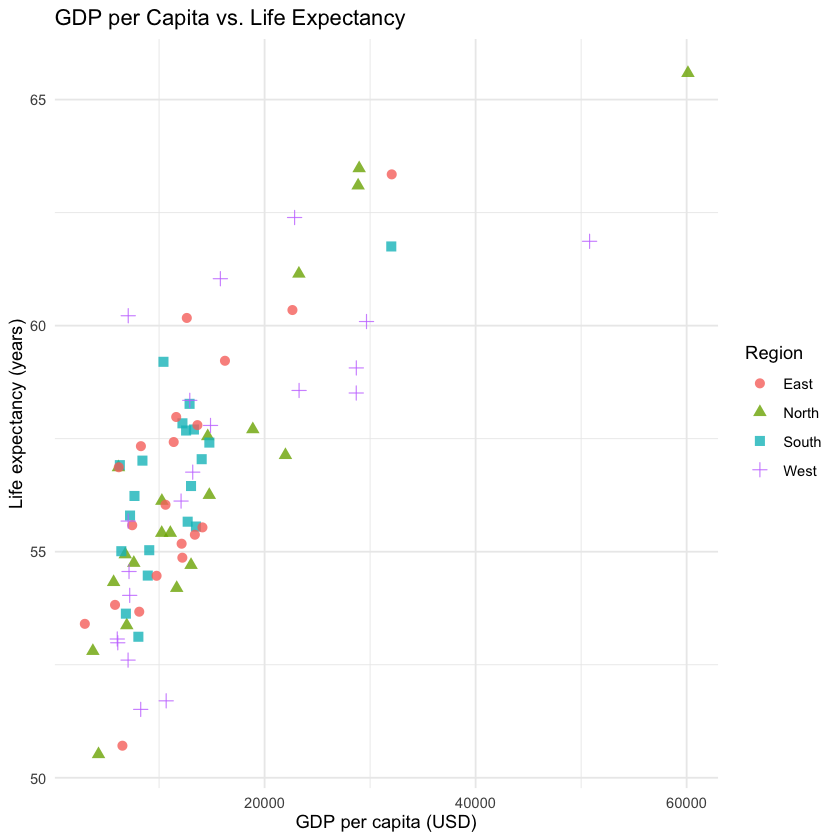
\includegraphics[width=4.375in,height=4.375in]{index_files/figure-latex/notebooks-notebook-02-fig-r-sample-output-1.png}

}

\caption{\label{fig-r-sample}Synthetic regional indicators: GDP per
capita vs.~life expectancy across 80 simulated regions, colored by
geographic cluster (R).}

\end{figure}%

\begin{table}

\caption{\label{tbl-r-summary}Summary statistics by region (R).}

\centering{

\begin{verbatim}


|Region | GDP mean|  GDP sd| Life exp. mean| Life exp. sd|  N|
|:------|--------:|-------:|--------------:|------------:|--:|
|East   |  11888.0|  6419.8|           56.5|          2.9| 20|
|North  |  15443.4| 13021.0|           56.8|          3.8| 20|
|South  |  11517.9|  5595.0|           56.6|          2.0| 20|
|West   |  15972.3| 11548.6|           56.8|          3.5| 20|
\end{verbatim}

}

\end{table}%

Although this notebook is straightforward, it highlights several
practical points for R users: configuring an R kernel in Jupyter,
sourcing a shared configuration file (\texttt{config.R}) for
reproducibility, and using R's visualization and table-formatting
ecosystem within the notebook environment. For researchers more
comfortable in R than Python, this notebook provides a familiar entry
point into the Jupyter workflow.

\section{Data Exploration in Stata}\label{sec-stata}

The third notebook (\href{notebooks/notebook-03.ipynb}{N3: Sample Stata
Analysis}) completes the multi-language comparison by performing the
same analysis in Stata. It uses the \texttt{nbstata} kernel, which
allows Stata commands to run directly inside Jupyter notebooks --- a
relatively recent development that brings Stata into the computational
notebook ecosystem.

The scatter plot below shows the GDP-life expectancy relationship using
Stata's \texttt{twoway\ scatter} graphics.

\begin{figure}[H]

\centering{

\pandocbounded{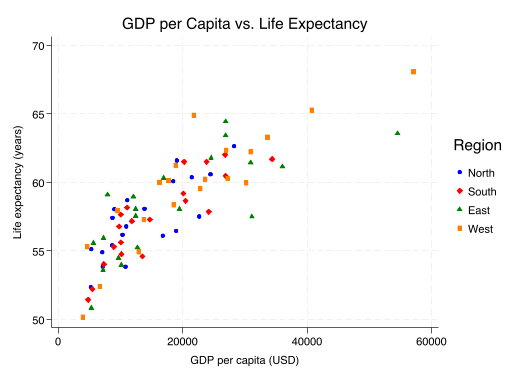
\includegraphics[keepaspectratio]{index_files/figure-latex/notebooks-notebook-03-fig-stata-sample-output-1.png}}

}

\caption{\label{fig-stata-sample}Synthetic regional indicators: GDP per
capita vs.~life expectancy across 80 simulated regions, colored by
geographic cluster (Stata).}

\end{figure}%

\phantomsection\label{stata-summary}
\begin{verbatim}

Summary statistics: Mean, SD, N
Group variable: region 

region |  gdp_pe~a  life_e~y
-------+--------------------
  East |   18540.3      58.2
       |   12777.3       3.7
       |      20.0      20.0
-------+--------------------
 North |   13941.3      57.3
       |    6845.2       2.8
       |      20.0      20.0
-------+--------------------
 South |   15757.6      57.4
       |    8297.8       3.1
       |      20.0      20.0
-------+--------------------
  West |   21923.5      59.7
       |   12889.5       4.3
       |      20.0      20.0
-------+--------------------
 Total |   17540.7      58.2
       |   10782.0       3.6
       |      80.0      80.0
----------------------------
\end{verbatim}

This notebook is particularly valuable for researchers who rely on Stata
for their primary analysis. It demonstrates that Stata users do not need
to abandon their preferred tool to benefit from the reproducibility and
documentation advantages of computational notebooks. The notebook covers
data generation with Stata syntax, graphing with \texttt{twoway}, and
summary statistics with \texttt{tabstat}.

\section{Machine Learning with Random Forest}\label{sec-ml}

The fourth notebook (\href{notebooks/notebook-04.ipynb}{N4: Introduction
to Machine Learning --- Random Forest Regression}) moves beyond
exploratory analysis to introduce a complete machine learning workflow
in Python. It predicts Bolivia's Municipal Sustainable Development Index
(IMDS) from 64-dimensional satellite image embeddings using Random
Forest regression.

\subsection{Target variable}\label{target-variable}

The IMDS scores across 339 municipalities range from 0 to 100 and follow
a roughly bell-shaped distribution with a slight right skew (mean =
51.1, median = 50.5).

\begin{figure}[H]

\centering{

\pandocbounded{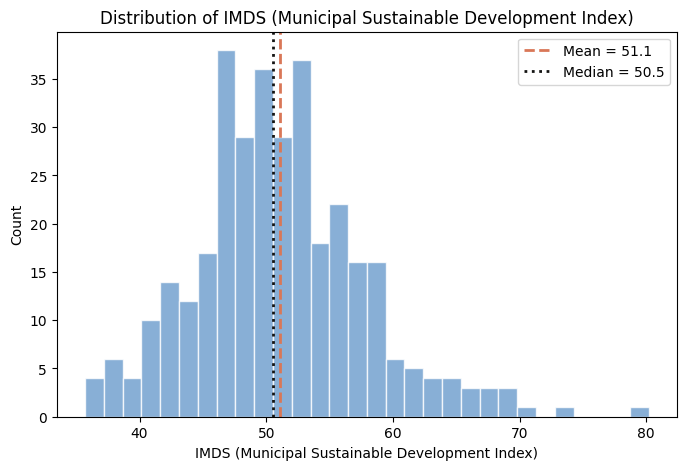
\includegraphics[keepaspectratio]{index_files/figure-latex/notebooks-notebook-04-fig-target-distribution-output-1.png}}

}

\caption{\label{fig-target-distribution}Distribution of IMDS scores
across Bolivia's municipalities. The dashed line marks the mean, the
dotted line marks the median.}

\end{figure}%

\subsection{Model performance}\label{model-performance}

The dataset is split into 271 training and 68 test municipalities. A
baseline Random Forest model is trained with 5-fold cross-validation,
followed by hyperparameter tuning via randomized search over 50
parameter combinations. The table below compares the baseline and tuned
models on the held-out test set.

\begin{longtable}[]{@{}lrr@{}}

\caption{\label{tbl-ml-results}Random Forest regression results:
baseline vs tuned model performance on the test set.}

\tabularnewline

\toprule\noalign{}
Metric & Baseline & Tuned \\
\midrule\noalign{}
\endhead
\bottomrule\noalign{}
\endlastfoot
R² & 0.2307 & 0.2297 \\
RMSE & 6.52 & 6.52 \\
MAE & 4.68 & 4.72 \\

\end{longtable}

Both models achieve an R-squared of approximately 0.23 and an RMSE of
about 6.5 points, indicating that satellite embeddings capture
meaningful but limited development signals. The scatter plot of actual
versus predicted values illustrates the typical regression-to-the-mean
pattern.

\begin{figure}[H]

\centering{

\pandocbounded{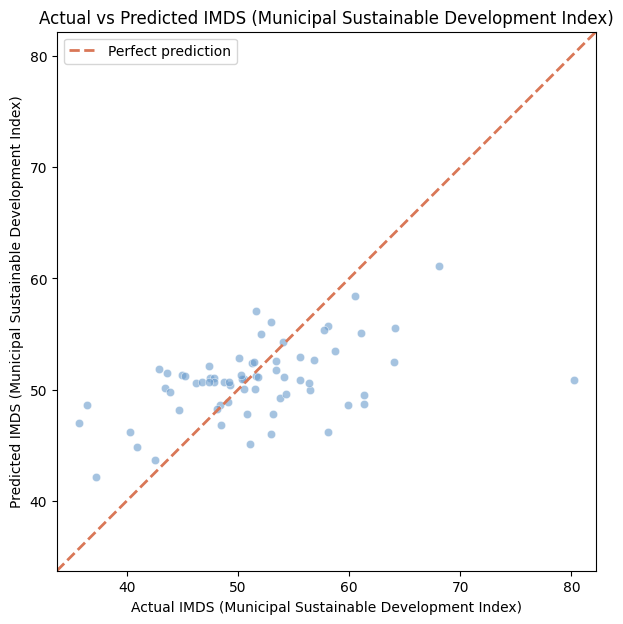
\includegraphics[keepaspectratio]{index_files/figure-latex/notebooks-notebook-04-fig-actual-vs-predicted-output-1.png}}

}

\caption{\label{fig-actual-vs-predicted}Actual vs predicted IMDS scores
on the test set. The dashed line represents perfect prediction.}

\end{figure}%

\subsection{Feature importance}\label{feature-importance}

A key advantage of Random Forest models is their interpretability
through feature importance measures. The permutation importance plot
below shows the top features ranked by their contribution to predictive
accuracy.

\begin{figure}[H]

\centering{

\pandocbounded{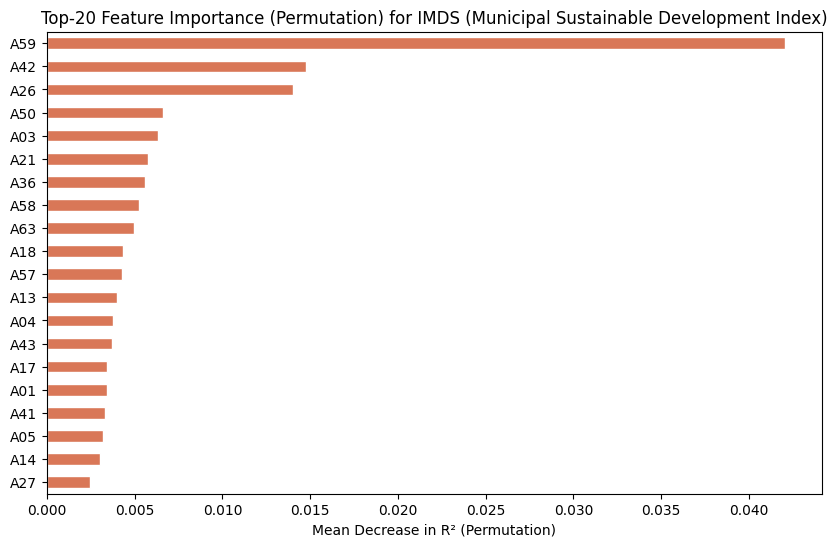
\includegraphics[keepaspectratio]{index_files/figure-latex/notebooks-notebook-04-fig-importance-permutation-output-1.png}}

}

\caption{\label{fig-importance-permutation}Top-20 satellite embedding
features ranked by permutation importance (mean decrease in R² when
feature is shuffled).}

\end{figure}%

Importance is distributed across many embedding dimensions rather than
concentrated in a few, suggesting that multiple aspects of the satellite
imagery contribute to predicting sustainable development outcomes.

\subsection{Partial dependence}\label{partial-dependence}

Partial dependence plots reveal non-linear relationships between
individual features and the predicted IMDS. Several features exhibit
threshold effects where the marginal relationship changes at specific
values.

\begin{figure}[H]

\centering{

\pandocbounded{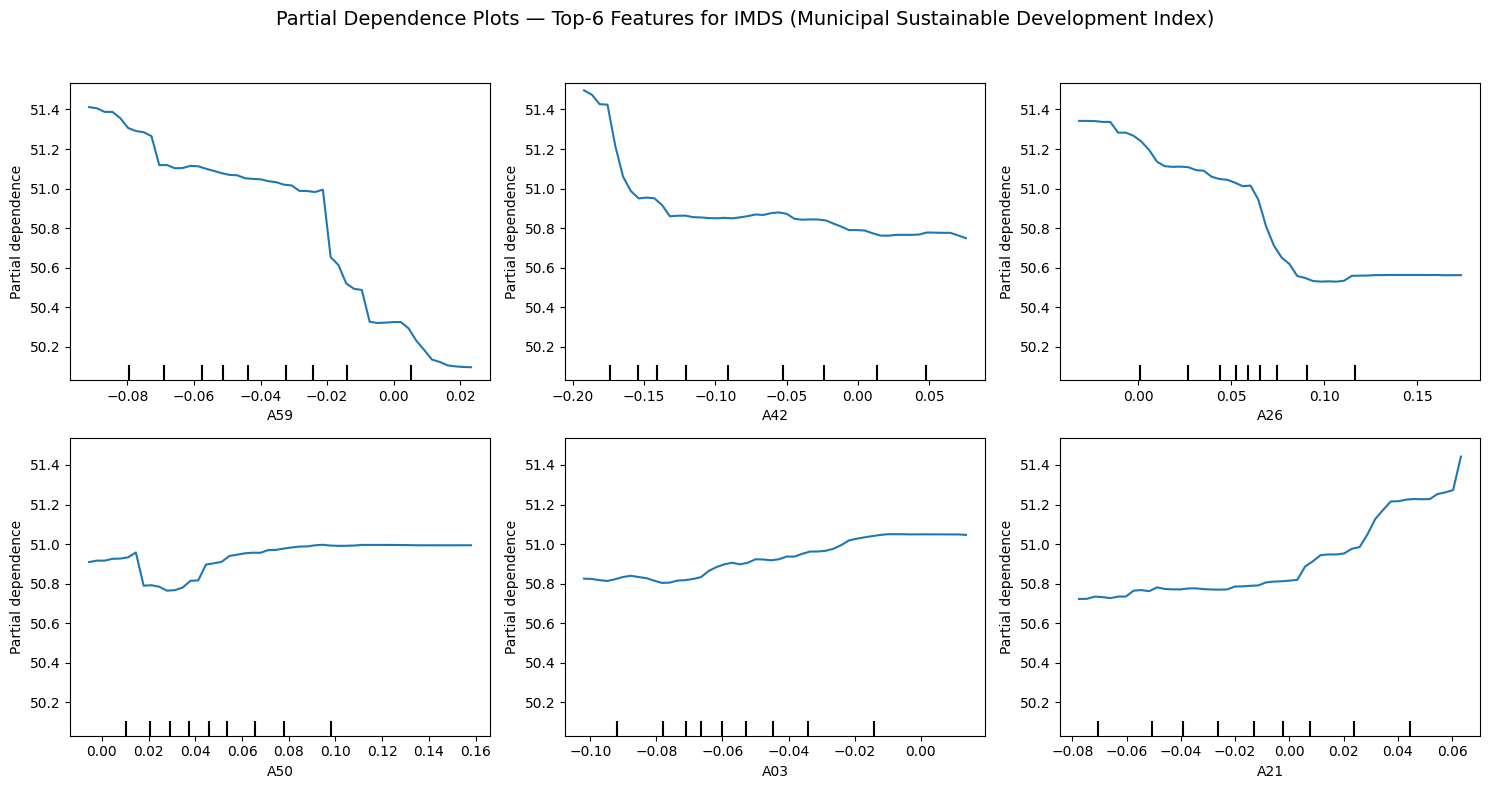
\includegraphics[keepaspectratio]{index_files/figure-latex/notebooks-notebook-04-fig-partial-dependence-output-1.png}}

}

\caption{\label{fig-partial-dependence}Partial dependence plots for the
top-6 most important satellite embedding features, showing how each
feature's value affects the predicted IMDS score.}

\end{figure}%

For full details on the methodology and hyperparameter search, see the
\href{notebooks/notebook-04.ipynb}{complete notebook}.

\section{Causal Inference with Double Machine
Learning}\label{sec-causal}

The fifth notebook (\href{notebooks/notebook-05.ipynb}{N5: Introduction
to Causal Inference --- Double Machine Learning}) introduces causal
inference methods using the Pennsylvania Reemployment Bonus experiment
as a case study. It demonstrates how Double Machine Learning (DoubleML)
corrects for the confounding bias that affects naive regression
estimates.

\subsection{The research question}\label{the-research-question}

The central question is whether offering a cash bonus to unemployed
workers causally reduces the duration of unemployment. The dataset
includes 5,099 workers --- 3,354 in the control group and 1,745 who
received the bonus treatment.

\begin{figure}[H]

\centering{

\pandocbounded{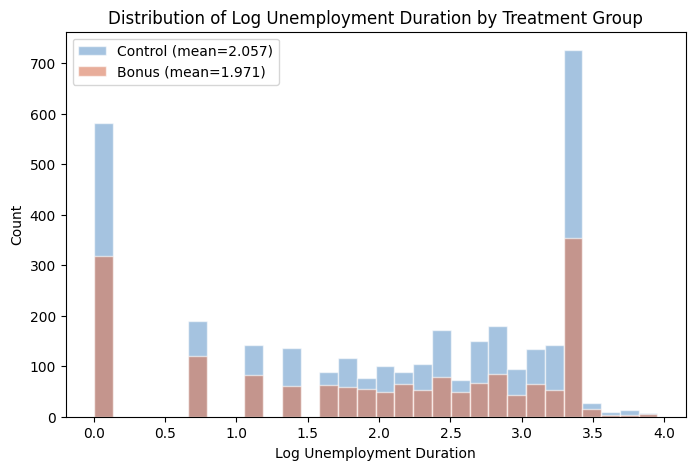
\includegraphics[keepaspectratio]{index_files/figure-latex/notebooks-notebook-05-fig-outcome-by-treatment-output-1.png}}

}

\caption{\label{fig-outcome-by-treatment}Distribution of log
unemployment duration by treatment group. The bonus group shows a
slightly lower mean.}

\end{figure}%

\subsection{Comparing estimation
methods}\label{comparing-estimation-methods}

The notebook compares four estimation approaches: naive OLS (without
covariates), OLS with covariates, DoubleML with Random Forest learners,
and DoubleML with Lasso learners. Naive OLS overestimates the treatment
effect by approximately 17\% compared to the debiased DoubleML
estimates.

\begin{figure}[H]

\centering{

\pandocbounded{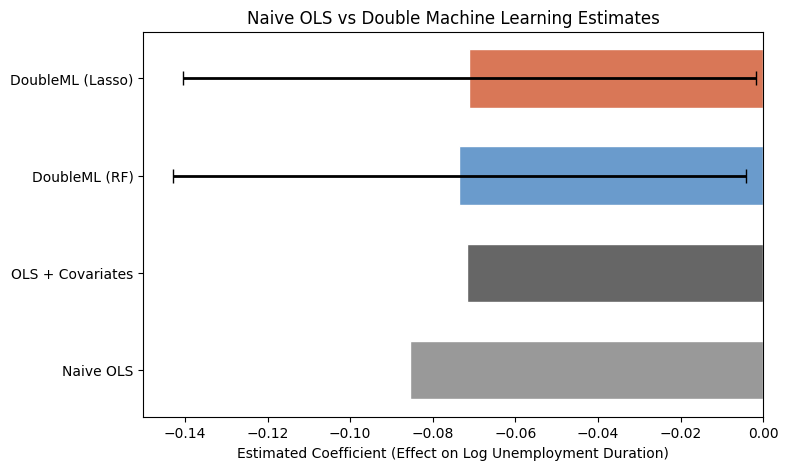
\includegraphics[keepaspectratio]{index_files/figure-latex/notebooks-notebook-05-fig-coefficient-comparison-output-1.png}}

}

\caption{\label{fig-coefficient-comparison}Comparison of causal effect
estimates across methods. Error bars show 95\% confidence intervals for
DoubleML methods.}

\end{figure}%

\subsection{Results}\label{results}

The DoubleML estimates indicate that the bonus reduces log unemployment
duration by approximately 0.07 (about 7\%), and this effect is
statistically significant. The table below summarizes the results across
all methods.

\begin{longtable}[]{@{}
  >{\raggedright\arraybackslash}p{(\linewidth - 8\tabcolsep) * \real{0.2338}}
  >{\raggedleft\arraybackslash}p{(\linewidth - 8\tabcolsep) * \real{0.1948}}
  >{\raggedright\arraybackslash}p{(\linewidth - 8\tabcolsep) * \real{0.1688}}
  >{\raggedright\arraybackslash}p{(\linewidth - 8\tabcolsep) * \real{0.1429}}
  >{\raggedright\arraybackslash}p{(\linewidth - 8\tabcolsep) * \real{0.2597}}@{}}

\caption{\label{tbl-doubleml-results}Comparison of treatment effect
estimates across methods.}

\tabularnewline

\toprule\noalign{}
\begin{minipage}[b]{\linewidth}\raggedright
Method
\end{minipage} & \begin{minipage}[b]{\linewidth}\raggedleft
Coefficient
\end{minipage} & \begin{minipage}[b]{\linewidth}\raggedright
Std Error
\end{minipage} & \begin{minipage}[b]{\linewidth}\raggedright
p-value
\end{minipage} & \begin{minipage}[b]{\linewidth}\raggedright
95\% CI
\end{minipage} \\
\midrule\noalign{}
\endhead
\bottomrule\noalign{}
\endlastfoot
Naive OLS & -0.0855 & --- & --- & --- \\
OLS + Covariates & -0.0717 & --- & --- & --- \\
DoubleML (RF) & -0.0736 & 0.0354 & 0.0378 & {[}-0.1430, -0.0041{]} \\
DoubleML (Lasso) & -0.0712 & 0.0354 & 0.0445 & {[}-0.1406, -0.0018{]} \\

\end{longtable}

The confidence intervals for the DoubleML estimates lie entirely to the
left of zero, confirming statistical significance. The results are
robust across different ML learners (Random Forest and Lasso).

\begin{figure}[H]

\centering{

\pandocbounded{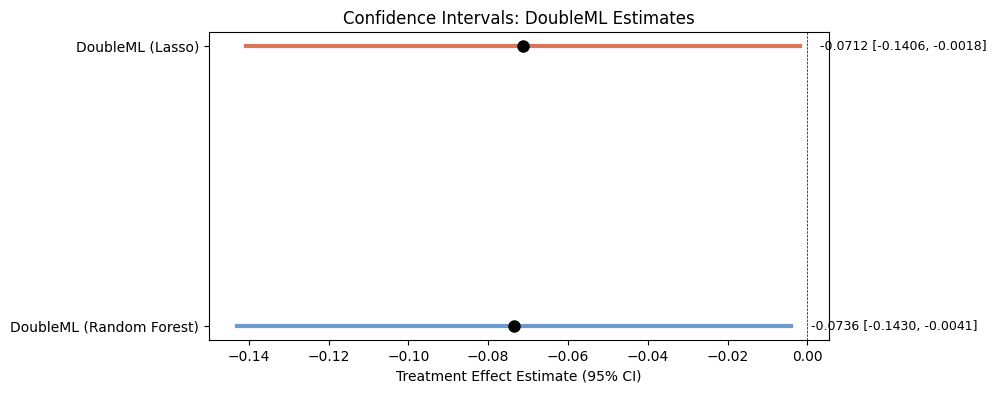
\includegraphics[keepaspectratio]{index_files/figure-latex/notebooks-notebook-05-fig-confint-output-1.png}}

}

\caption{\label{fig-confint}95\% confidence intervals for the DoubleML
causal effect estimates using two different ML learners.}

\end{figure}%

For the full methodological treatment --- including the Partially Linear
Regression framework, cross-fitting procedure, and discussion of
assumptions --- see the \href{notebooks/notebook-05.ipynb}{complete
notebook}.

\section{Concluding Remarks}\label{sec-conclusion}

This document has introduced five computational notebooks spanning three
programming languages and three analytical approaches:

\begin{itemize}
\tightlist
\item
  \textbf{Notebooks 1--3} demonstrate that Python, R, and Stata can all
  operate within the Jupyter notebook environment, producing comparable
  results for the same exploratory analysis task. This lowers barriers
  for researchers who prefer one language but want the benefits of
  reproducible, self-documenting workflows.
\item
  \textbf{Notebook 4} provides a hands-on introduction to machine
  learning with Random Forest regression, showing how satellite image
  embeddings can predict municipal development outcomes --- explaining
  approximately 23\% of the variance in Bolivia's IMDS.
\item
  \textbf{Notebook 5} introduces causal inference with Double Machine
  Learning, illustrating how debiased estimation corrects for
  confounding bias relative to naive OLS approaches.
\end{itemize}

Together, these notebooks serve as a practical reference for researchers
and students learning to work with computational notebooks across
multiple programming environments.

\section{Acknowledgments}\label{acknowledgments}

This research uses data from the
\href{https://github.com/quarcs-lab/ds4bolivia}{DS4Bolivia} project. The
analytical workflow was developed at Nagoya University.

\section{Data and Code Availability}\label{data-and-code-availability}

The data and code used in this study are available at
\url{https://github.com/quarcs-lab/ds4bolivia}. All notebooks are fully
reproducible using the \texttt{uv} environment manager and the
dependencies specified in \texttt{pyproject.toml}.

\section*{References}\label{references}
\addcontentsline{toc}{section}{References}




\end{document}
